\chapter{Methodology}

Students participated in five 90-minute activity sessions, once per week, for five consecutive weeks. Each session presented one activity that was intended to exercise different engineering and design principles. Students were observed and video recorded as they carried out the activities. 

\section{Subject Selection} 

This study used seven middle-school students as subjects. Students were in grades seven and eight, with average age of approximately 12 years old.  The selection process was done by an after school enrichment program, where this study was advertised as an activity students could elect to participate in.  This study was open to all students of the specified grade levels. Selection was simply the first students to volunteer to participate.

All students read, understood, and signed a student assent form and their guardians read, understood, and signed a parental consent form. Parental consent forms were available in English and Spanish. The student assent form was available only in English, as that is the language the research activities were conducted in. Guardians had the option to sign a media release form, which allowed recorded media of their child to be used in publication. 

\section{Session Protocol}

In each session, students engaged in an engineering and design activity. Their conversations, problem-solving strategies, and concluding interviews were observed in person by researchers and video recorded. 

Each of the five sessions followed the same pattern. Students arrived and were taken to a conference room for snack time, where they were casually introduced to the concepts involved in that day's activity. Loud thinking TODO(ref) was explained and reinforced every week at this time. After about twenty minutes in the conference room, the students moved to the activity room where the apparatus for that day's study was set up. Working in pairs, students worked through the prescribed activity. The entire time in the activity room was  audio and video recorded. Throughout the activity students were prompted by researchers to explain their thoughts, ideas, and understanding of concepts.

At the conclusion of the activity, students were lead in a group conversation about what they learned and developed. The questions asked by researchers during this conversation were variations of this set:
\begin{itemize}
\item What did you do to find your solution?
\item Did you do anything early on that you did again to help yourself?
\item If you had a friend who was coming in to work on this problem tomorrow,
what would you recommend they do? (Keep in mind the problem won't
have the exact same solution.)
\item Are there any other tricks you discovered?
\end{itemize}


%%%%%%%%%%%%%%%%%%%%%%%%%%%%%%%%%%%%%%%%%%%
%%%%%%%%%%%%%%%%%%%%%%%%%%%%%%%%%%%%%%%%%%%
\section{Design of Activities} TODO

The activities performed by the students were designed progressively, so each activity was informed by the performance of the previous. Each activity stressed different areas of engineering space, starting with a simple activity and progressing towards computational thinking, as defined by \citet{p33-wing}.
Subject areas of activities include:
\begin{itemize}
\item Math problem solving
\item Parallel and series circuits
\item Gear ratios and reduction
\item Algorithm design
\item String-matching 
\item Active control systems
\end{itemize}
In addition to subject areas, the activities will stress different
elements of design skills:
\begin{itemize}
\item Balancing between contradicting requirements
\item Working in time constraints
\item Physical construction
\item Symbolic manipulation of a system
\end{itemize}

%%%%%%%%%%%%%%%%%%%%%%%%%%%%%%%%%%%%%%%%%%%Rush Hour
\subsection{Week 1: Rush Hour}
	
	\textquotedblleft{}Rush Hour\textquotedblright{} is a sliding tile game where the player must manipulate cars on a small grid. The game has a small set of simple rules, but a high number of possible states for any given puzzle. The object of the game is to slide the target car, indicated in Figure \ref{fig:rushhourgame} by the arrow, out of the grid through the opening to the right of the game board. 
	
	%
	\begin{figure}
	\begin{centering}
	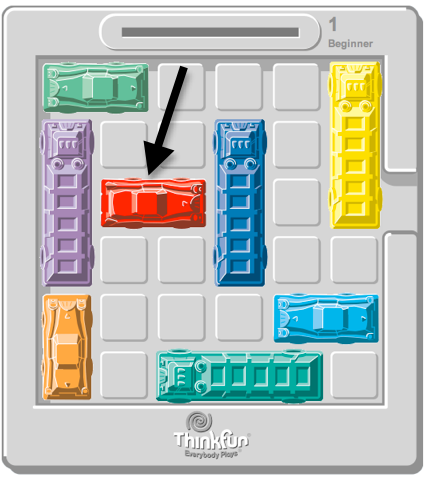
\includegraphics[height=0.35\textheight]{images/rushour-2}
	\par\end{centering}
	
	\caption{Rush Hour game board. The arrow indicates the target car.}
	\label{fig:rushhourgame}
	\end{figure}
	
	\subsubsection{Purpose}
	
	This activity was an ideal introductory experience for the students. It had very few rules to learn and was fun to play. Students were quickly engaged. As a design activity, this provided observations of the students' methods in navigating the deep state space of the game. With every move of a game piece the possible states accessible on the next move change. Many times the path the player is on does not have a solution anywhere on it, and the player must backtrack to reach an earlier state where a different decision could yield a solution, or, start over and try again. This backtracking was a primary component of the analysis of this activity.
	
	Welch cites \citet{ericsson-1984} with the importance of a warm up process, stating that when verbal information exchange is involved a period of warm-up is necessary for the subject and researcher to communicate most effectively. This activity, with such simple rules, provided an opportunity for students to focus on the loud thinking strategy, warming up that skill for the remaining sessions.
	
	\subsubsection{Protocol}
	
	The students were each given a game unit with a beginner level puzzle to solve.  The students were encouraged to {}``think out loud'' during the entire process, and to think about the process they were employing to arrive at solutions.
	
	Once the students felt that they understand the concept of the game, they were put into pairs and given a more difficult puzzle. The students\textquoteright{} process of solving this puzzle was video and audio recorded. The camera was positioned above the table to record the game board, the students\textquoteright{} hands,
	and the students\textquoteright{} voices. Additional puzzles of increasing difficulty were used as time allowed.
	
	At the conclusion of the puzzle solving session the students pairs were asked to explain the process of solving the puzzle. The students were instructed to explain their process of finding a solution, not the steps to carry out a specific solution. They were then instructed to explain the game strategy for a friend who has not seen the game before.
	
	A semi-structured interview was used to probe students\textquoteright{} understanding. The interview was based on these questions:
	\begin{itemize}
	\item Please explain what you did to find the solution to these puzzles. 
	\item Did you do anything in the first puzzle that you did again in the
	second to help yourself out? 
	\item I want you to explain how to go about solving these kinds of puzzles.
	Pretend you\textquoteright{}re explaining it to a friend who has never
	done this before. 
	\item Are there any tricks you discovered? 
	\end{itemize}
	
	\subsubsection{Rationale}
	
	This game is characterized by its large state space, rapid iteration of ideas, and high level of backtracking. This type of problem is common, and can be generalized to include other games (such as chess) as well as real engineering problems. For example, circuit board routing is a design activity that has a large number of states where decisions progressively lead to new areas of the state map, fitting this general problem type.

%%%%%%%%%%%%%%%%%%%%%%%%%%%%%%%%%%%%%%%%%%%Lights
\subsection{Week 2: Light \& Power Optimization}

	Students were presented small light bulbs connected in a certain
	configuration with a power supply. Their design task is to reduce
	the number of wires necessary to light all the bulbs without significant
	sacrifice in brightness. This problem explores basic electrical principles
	and requires students to balance between contradicting requirements.
	The students were given a story that they work for a power company,
	and each light bulb represents a house on their grid. They need to
	find a method to light all of the homes at the lowest cost to the
	company.
	
	
	\subsubsection{Purpose}
	
	This activity will generate observations of students exploring natural
	phenomena and balancing requirements for an optimal solution. The
	definition of optimal was left partially open, allowing students
	to construct arguments for the optimality of their solution, which
	will further promote loud thinking and give insight to the student's
	thought processes.
	
	
	\subsubsection{Protocol}
	
	During snack time, a researcher will lead a conversation about what
	{}``optimization'' means, soliciting suggestions from the students.
	Once in the classroom, the students were presented with a workstation
	for each dyad. Each workstation will have a variable DC power supply,
	a number of small, low-power light bulbs (holiday mini-bulbs), and
	connecting wires with alligator clips. Two workstations were initially
	set up with example circuits. One was a number of lights connected
	in series, such that the same current flow runs through all the lights,
	with the power supply operating at 12 volts. The other station will
	have the same number of lights connected in a parallel configuration,
	such that every light has full voltage from pole-to-pole on the power
	supply, which was operating at 3 volts. The two systems were
	approximately the same brightness. The terms {}``series'' and {}``parallel''
	are never used with the students.
	
	The students were presented with a set of criteria for assessing
	their solutions. The goal was stated to achieve {}``reasonable
	brightness.'' Costs were associated for number of wires used and
	amount of voltage required. The final cost of a solution was \[
	\frac{\alpha\cdot c+\beta\cdot v}{n}\]
	where $c$ is the number of connection wires, $v$ is the voltage
	being supplied, and $n$ is the number of light bulbs being serviced.
	The multipliers $\alpha$ and $\beta$ are the respective costs of
	wires and voltage.
	
	The students, working in pairs, will solve two iterations of this
	activity. The two iterations will have different material costs. The
	change in cost values was designed to obsolete the first iteration's
	optimal solution, forcing reconsideration of the problem.
	
	At the conclusion of the second problem iteration, the students, in
	pairs, were asked to document their solutions and explain how they
	arrived at them. They were instructed to explain their process
	as if for a friend who was not present. Interview questions will examine
	the students grasp of the electrical principles, what they considered
	to be {}``optimal,'' and how they went about discovering what they
	needed to know in order to solve the problem.
	
	
	\subsubsection{Rationale}
	
	The electrical concepts in this activity are fundamental to an understanding
	of electricity and electronics, and create the physical basis of computing
	technology. The problem is also multi-dimensional, with number of
	connections, voltage, and number of lights serving as related but
	axiomatically confounded design parameters \citet{axiomatic}. This
	activity emulates real-world design problems that requires simplification,
	satisficing, or constraint of solution space.

%%%%%%%%%%%%%%%%%%%%%%%%%%%%%%%%%%%%%%%%%%%Gears
\subsection{Week 3: Gear Reduction}

	In this activity the students will build a transmission from Lego
	Technic gears and components between a fixed motor and load. 
	
	
	\subsubsection{Purpose}
	
	This problem allows for direct access to the students' spatial and
	mechanical reasoning skills, a domain used heavily in many different
	areas of design.
	
	
	\subsubsection{Protocol}
	
	The students were introduced to the concepts of gear reduction,
	specifically the nature of {}``little-to-big'' relationships \citet{ArtofLEGO}.
	Each student dyad was supplied with a workstation apparatus, constructed
	of Lego Technic with a motor, a large wall on which to build their
	transmission, and an output pulley. The pulley was connected to
	an interchangeable mass. The students are presented with two different
	tasks, and they may attempt one or both:
	\begin{enumerate}
	\item Lift the greatest amount of weight possible.
	\item Lift a specific weight from the floor as quickly as possible.
	\end{enumerate}
	The students will have all the remaining time to design and build
	their solutions. Paper was provided, and students were encouraged
	to document their transmissions in the same fashion as was used in
	the concept tutorial.
	
	At the conclusion of the work time, each dyad's construction will
	be tested individually as the group observes.
	
	
	\subsubsection{Rationale}
	
	This activity is very purely an engineering design task. The requirements,
	constraints, and success criteria are extremely clear. The solution,
	however, is open-ended, as the gears can be assembled in nearly infinite
	configurations, many of which may solve the problem. This activity
	stresses implementation and time management.

%%%%%%%%%%%%%%%%%%%%%%%%%%%%%%%%%%%%%%%%%%%Word Search
\subsection{Week 4: Word Search}

	Students will design algorithms to solve word searches, where words
	are hidden in a two-dimensional grid of otherwise random letters.
	This activity will introduce the concepts of pseudocode and flowcharts
	for algorithm design.
	
	
	\subsubsection{Purpose}
	
	The concept of an algorithm was introduced in this activity, which
	will also be used in the following activity. As such, this activity
	will partially function as a warm up to the more complex elevator
	control algorithm activity. 
	
	This activity will allow observations of students process in deducing
	and applying patterns, and observe students' approaches to writing
	generalized procedures.
	
	
	\subsubsection{Protocol}
	
	This protocol was implemented as a worksheet for students, as can
	be seen in Appendix \ref{sec:wordsearchhandout}. The concept of an
	algorithm was introduced with the game of tic-tac-toe as example.
	The students were given the instruction set to never lose tic-tac-toe,
	and are encouraged to study and try it. Once the concept of using
	instructions to play a game has been mastered, the students were
	given a very simple word search puzzle. The example puzzle was
	designed to be nearly trivial, like the one in Figure \ref{fig:Example-word-search}.
	The words hidden in this puzzle are \emph{ace}, \emph{fire}, \emph{shoe},
	\emph{tour}, and \emph{yes}.
	
	\begin{center}
	%
	\begin{figure}
	\begin{centering}
	\begin{tabular}{|c|c|c|c|c|}
	\hline 
	Y & E & S & L & F\tabularnewline
	\hline
	\hline 
	M & N & H & R & I\tabularnewline
	\hline
	\hline 
	P & T & O & U & R\tabularnewline
	\hline
	\hline 
	A & C & E & M & E\tabularnewline
	\hline
	\end{tabular}
	\par\end{centering}
	
	\caption{\label{fig:Example-word-search}Example word search puzzle.}
	
	
	
	\end{figure}
	
	\par\end{center}
	
	The students were prompted at this point with questions, which
	were discussed briefly as a group. The questions were:
	\begin{itemize}
	\item Did you find all the words?
	\item What did you do to find the words?
	\item Did the words just {}``jump out at you?'' 
	
	\begin{itemize}
	\item What if they didn't?
	\item How can you know for sure you found \emph{all} the words?
	\end{itemize}
	\end{itemize}
	The students will then be prompted to write down any rules or strategies
	they employed in the example puzzle. 
	
	The researcher will explain that computers are devoid of the pattern
	recognition ability that makes words {}``jump out'' for people.
	However, computers are very fast at simple computation, so they are
	advantageous to use for extremely large data sets. This should provide
	impetus for the students to develop an algorithm rather than simply
	solve the puzzle one time.
	
	The students will then be given the difficult puzzle, which can be
	seen in Appendix \ref{sec:wordsearchpuzzle}. The students were encouraged
	to continue talking through their thought process, and reminded that
	the process to solve the problem is desired, not the solution itself.
	If the students complete the puzzle and are confident in the rules
	they have written, they were given an additional puzzle with the
	instructions to solve it only by following their rules, not using
	their human abilities.
	
	
	\subsubsection{Rationale}
	
	This activity will stress computational thinking,
	causing students to think algorithmically about a normally straightforward
	task. This activity also has opportunity for cleverness and creativity
	that may arise from noticing patterns in data. These skills are fundamental
	to computer science. 

%%%%%%%%%%%%%%%%%%%%%%%%%%%%%%%%%%%%%%%%%%%Elevator
\subsection{Week 5: Elevator Control}

	Students will design a set of rules to govern the motion of a simulated
	elevator. Elevators are robotic devices that need to act based on
	multiple inputs and system states, and require well-thought-out control
	algorithms to function effectively. The simulated elevator was
	implemented in Scratch \citet{scratch} using BYOB \citet{byob},
	allowing for custom drag-and-drop code blocks for high-order control
	of the graphical elevator system.
	
	
	\subsubsection{Purpose}
	
	This activity will explore the students reactions to a difficult optimization
	problem. Students were observed developing the problem concept
	as well work towards improved solutions. Unique among the other sessions,
	in this activity students will also be observed working purely symbolically.
	
	
	\subsubsection{Protocol}
	
	The students were tasked with a simple goal: develop an algorithm
	to control an elevator. The concept of simulation was introduced,
	as will the Scratch programming language subset used by the simulator.
	The primary elevator control blocks can be seen in Figure \ref{fig:Elevator-blocks}.
	
	%
	\begin{figure}
	\begin{centering}
	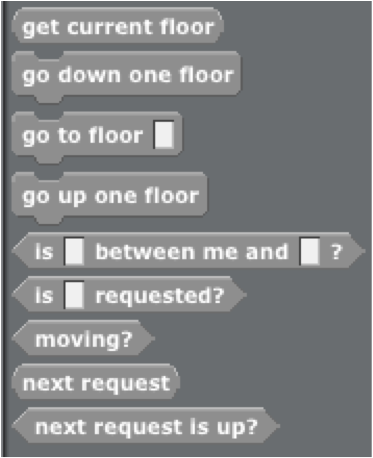
\includegraphics{images/elevator_primitives}
	\par\end{centering}
	
	\caption{\label{fig:Elevator-blocks}Elevator control blocks.}
	
	
	
	\end{figure}
	
	
	The students were provided with a trivial but working solution,
	shown in Figure \ref{fig:elevator-trivial}. The first challenge will
	be to understand why the givens solution works and why it is sub-optimal.
	There was no formal mechanism to prevent students from working
	on a solution before they fully understand the problem, but they will
	be prompted often by researchers to establish their current understanding
	of the situation.
	
	The provided solution simply travels to the next floor that it was
	called to, in the order that the calls were made. The major flaw of
	this solution is that people who are waiting for service were passed
	by the elevator as it travels blindly to whomever pressed the button
	first. This inefficiency would result in unacceptable wait times (and
	therefore unhappy people), as well as unnecessary energy expenditure
	by the building owner.
	
	%
	\begin{figure}
	\begin{centering}
	
\includegraphics{images/elevator-trivial-solution}
	\par\end{centering}
	
	\caption{\label{fig:elevator-trivial}Trivial solution of the elevator control
	problem.}
	
	
	
	\end{figure}
	
	
	
	\subsubsection{Rationale}
	
	This activity is highly abstracted, symbolic, and the problem is difficult
	to characterize. It also requires understanding of a queue structure,
	positional queries, and boolean logic. These elements are part of
	the everyday problems posed by both researching and practicing computer
	scientists and engineers. Control elements, such as determining location
	and direction of travel, are specifically common to robotics.




%%%%%%%%%%%%%%%%%%%%%%%%%%%%%%%%%%%%%%%%%%%Analysis
%%%%%%%%%%%%%%%%%%%%%%%%%%%%%%%%%%%%%%%%%%%Plan
\section{Analysis Plan}
Videos from student sessions were analyzed using coding techniques informed by \citet{welch}, where specific codes were defined to describe important behaviors. Additional codes were created as needed as informed by grounded theory. The additional codes allowed for behaviors and patterns that were not predicted to be documented as they were observed.

The initial code list was based on the codes used by \citet{REESE},
as that research has a similar experimental setup with a similar group
of subjects. The codes, in accordance with \citeauthor{REESE}, were categorized by stages of the design cycle. They are described in Table \ref{tab:Starting-codes}.


%
\begin{table}
\begin{centering}
\begin{tabular}{|c|c| p{3.5in} |}
\hline 
Design Step & Code & Definition\tabularnewline
\hline
Understand the problem & RB & Read design brief as given to the subjects by the researcher\tabularnewline
\cline{2-3} 
({}``ASK'') & DPER & Discussing/referring to performance criteria\tabularnewline
\cline{2-3} 
 & DCON & Discussing/referring to constraints\tabularnewline
\cline{2-3} 
 & PK & Accessing prior knowledge\tabularnewline
\cline{2-3} 
 & CAR & Check available resources\tabularnewline
\hline 
Generate possible solutions & DIS & Discussing possible solutions\tabularnewline
\cline{2-3} 
({}``IMAGINE'') & SBS & Selecting best solution\tabularnewline
\cline{2-3} 
 & MAN & Manipulation of materials to explore properties\tabularnewline
\hline
Modeling a possible solution & PP & Planning a prototype\tabularnewline
\cline{2-3} 
({}``PLAN'') & DRAW & Sketching/drawing possible solutions\tabularnewline
\cline{2-3} 
 & MP & Making a prototype\tabularnewline
\cline{2-3} 
 & TEST & Testing one element as the making continues\tabularnewline
\cline{2-3} 
 & AB & Abandon current solution; begin new solution\tabularnewline
\hline 
Building a solution & IP & Identify a problem with the prototype\tabularnewline
\cline{2-3} 
({}``CREATE'') & MDC & Making a design change to the prototype\tabularnewline
\cline{2-3} 
 & REF & Refining construction of prototype\tabularnewline
\hline 
Evaluation & EO & Evaluate as subjects observe prototype\tabularnewline
\cline{2-3} 
({}``IMPROVE'') & ET & Evaluate as subjects talk about prototype\tabularnewline
\cline{2-3} 
 & ED & Evaluate as subjects draw possible solution\tabularnewline
\cline{2-3} 
 & EDB & Evaluating in terms of the design brief\tabularnewline
\hline
\end{tabular}
\par

\end{centering} 

\caption{\label{tab:Starting-codes}Starting codes.}

\end{table}


This set of codes only provided a starting point for analysis. Additional codes were created as needed during analysis, and will be discussed in chapter \ref{chap:analysis}. 

Analysis was done primarily using NVIVO software. Codes were applied to specific time spans of the video where the corresponding behavior or activity was observed. Data
were analyzed both to see how the individual students changed over the period
of time (idiographic) and to see trends in all the students as a group
(nomothetic).

The plan of analysis was to find emergent patterns in the data consisting of video codes, researcher notes, and student products. 
